Escribe una expresión para calcular el perímetro y el área de la figura \ref{fig:20230319035140}

\begin{figure}[H]
    \centering
    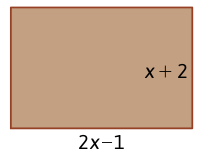
\includegraphics[width=0.25\textwidth]{../images/20230319035140}
    \caption{}
    \label{fig:20230319035140}
\end{figure}


\begin{solutionbox}{3.5cm}
    \begin{multicols}{2}
      Perímetro:
      \begin{align*}
        P & =2(2x-1)+2(x+2) \\
          & =4x-2+2x+4     \\
          & =6x+2
      \end{align*}
  
      Área:
      \begin{align*}
        A & =(2x-1)(x+2)     \\
          & =2x^2+3x-2
      \end{align*}
    \end{multicols}
  \end{solutionbox}